\section{Examples and comparison}


\begin{frame}
	\frametitle{Comparison with KDL Symmetric Velocity profiles}
	\hglue -1cm
	\begin{tikzpicture}[scale=1, transform shape]
		\node[anchor=north west](pic){%
			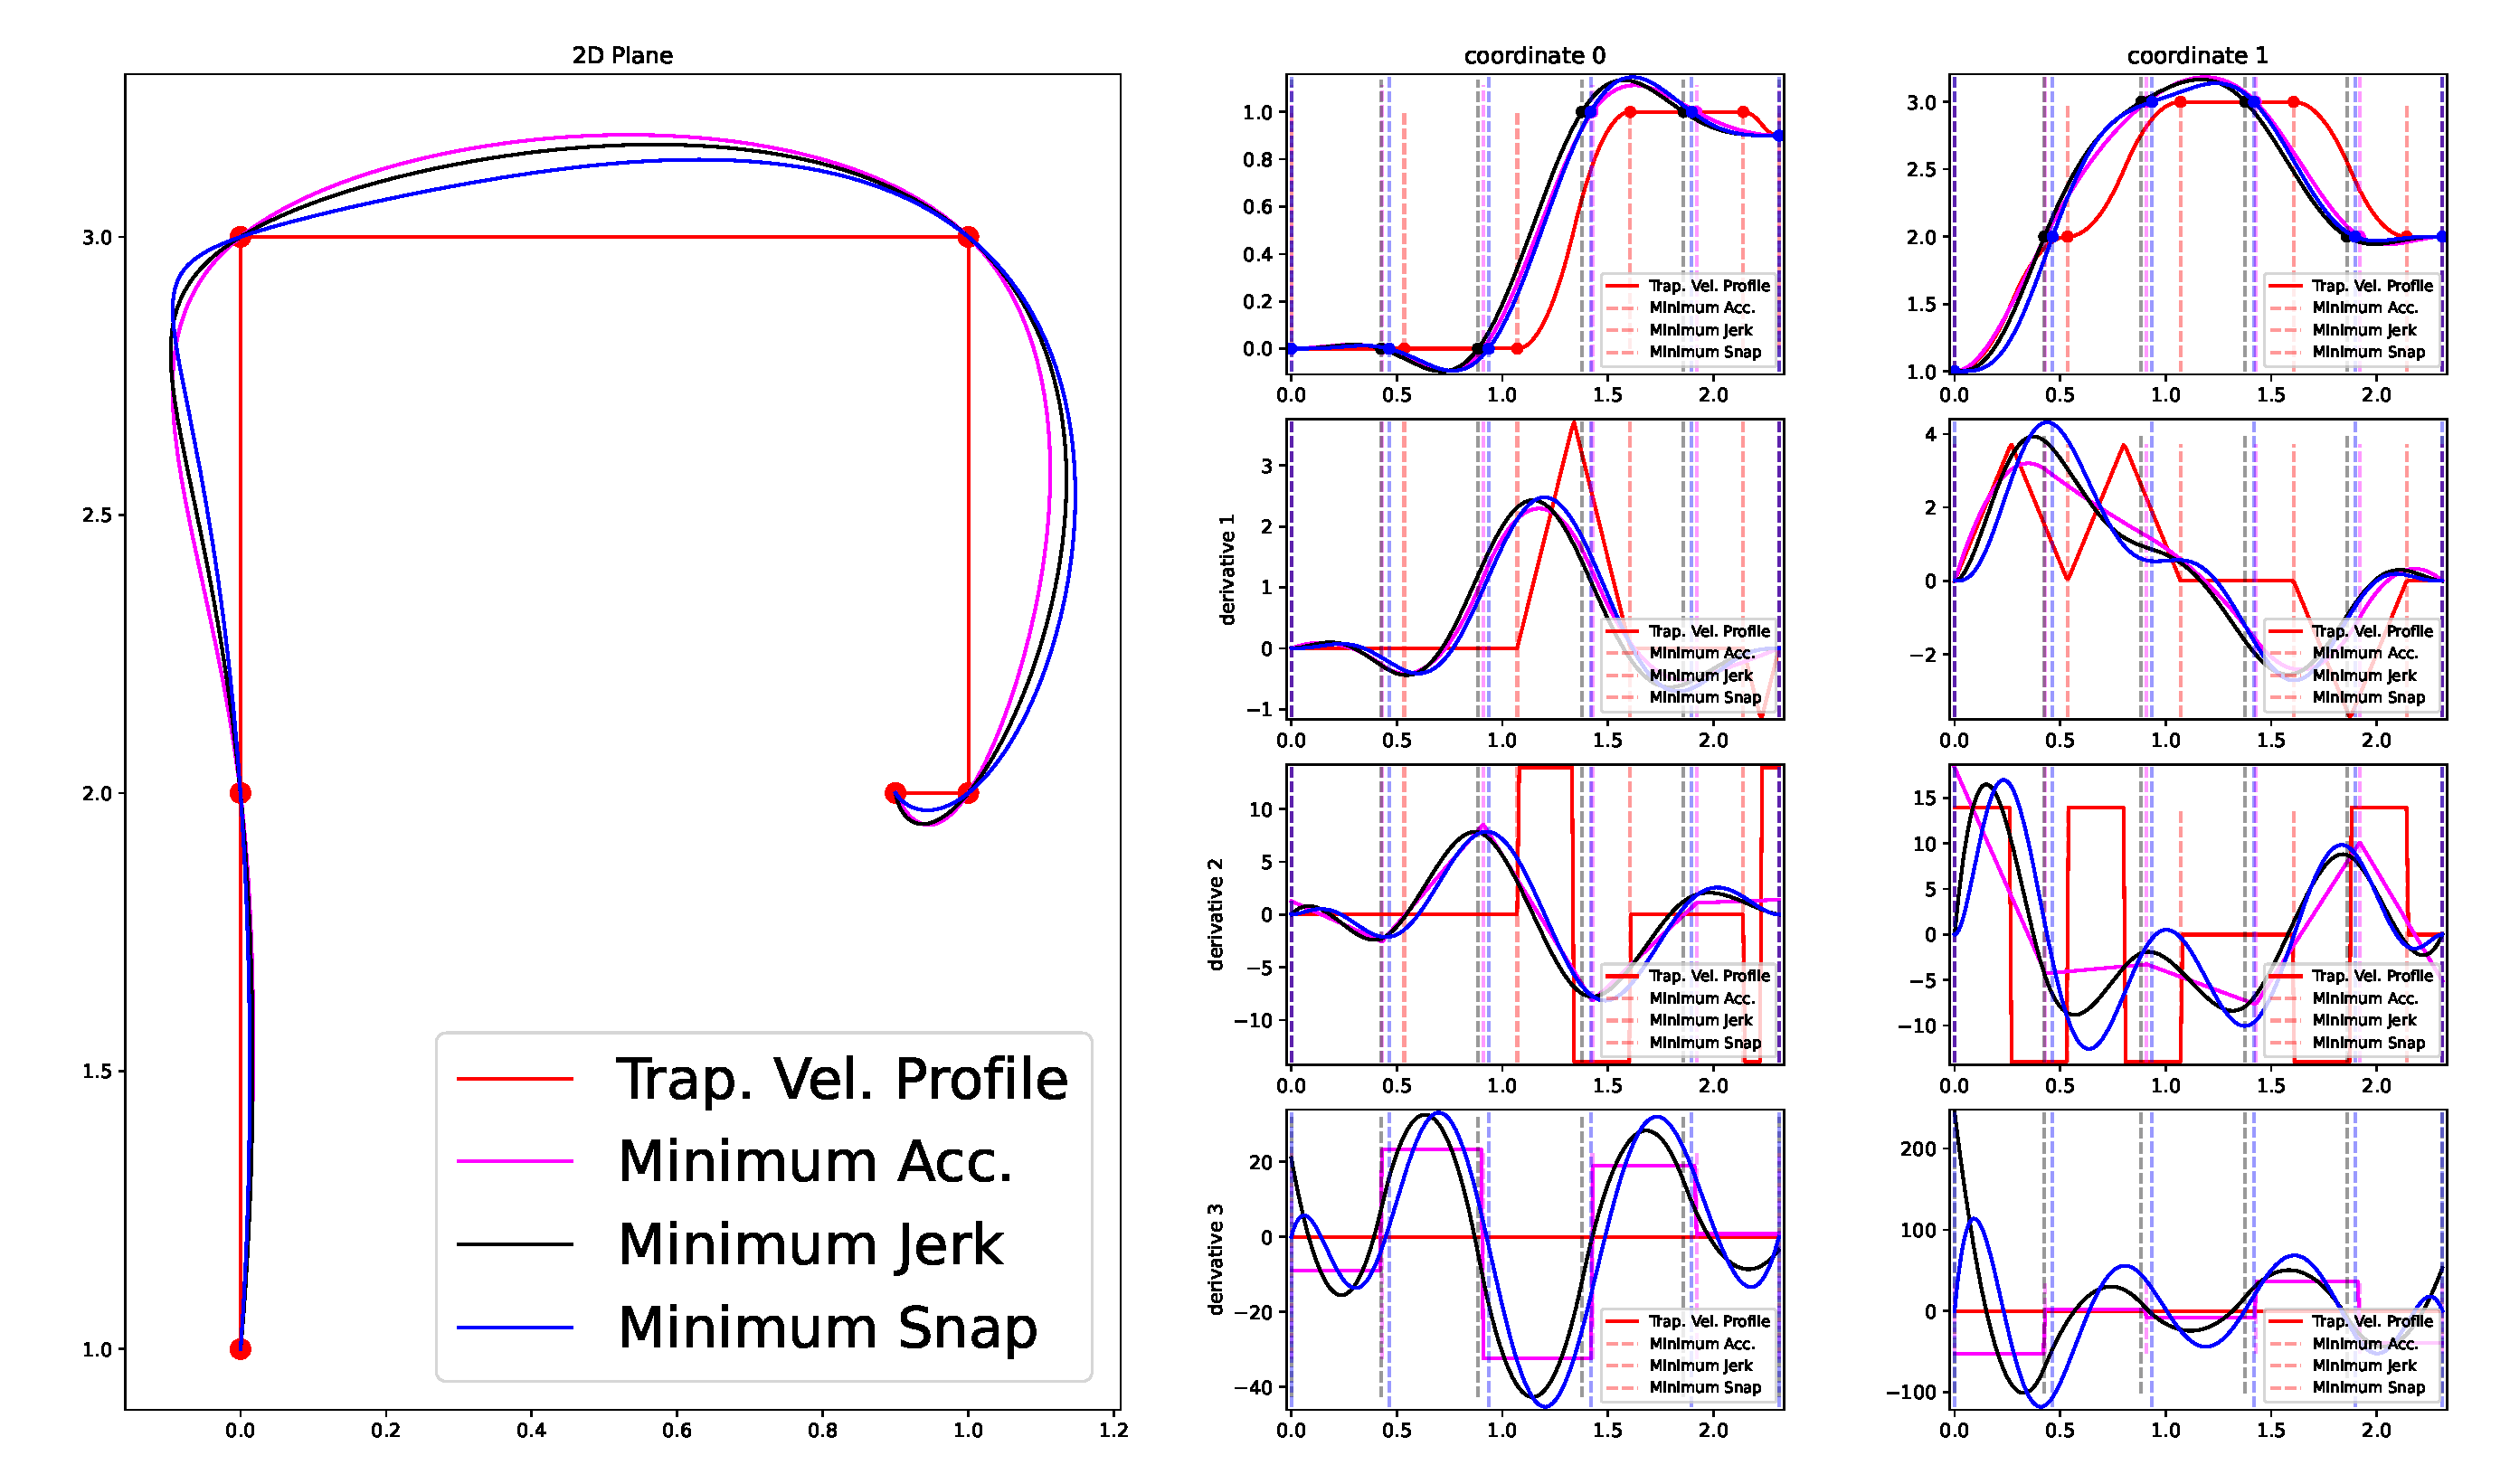
\includegraphics[width=10cm]{./images/kdl_comparision_1.pdf}};
		\node[anchor=west, text width=5cm] (title) at (pic.east){%
			\emphImFusion{Remark:}
			Minimum-X trajectories
			present large overshoots.
			As the arc-lenght is larger, this trajectores are slower
		};
	\end{tikzpicture}

\end{frame}

\begin{frame}
	\frametitle{Comparison with KDL Symmetric Velocity profiles}
\end{frame}

\begin{frame}
	\frametitle{Comparison with KDL Symmetric Velocity profiles}
	\framesubtitle{Overshoot reductions}
	\hglue -1cm
	\begin{tikzpicture}[scale=1]
		\node[anchor=north west](pic){%
			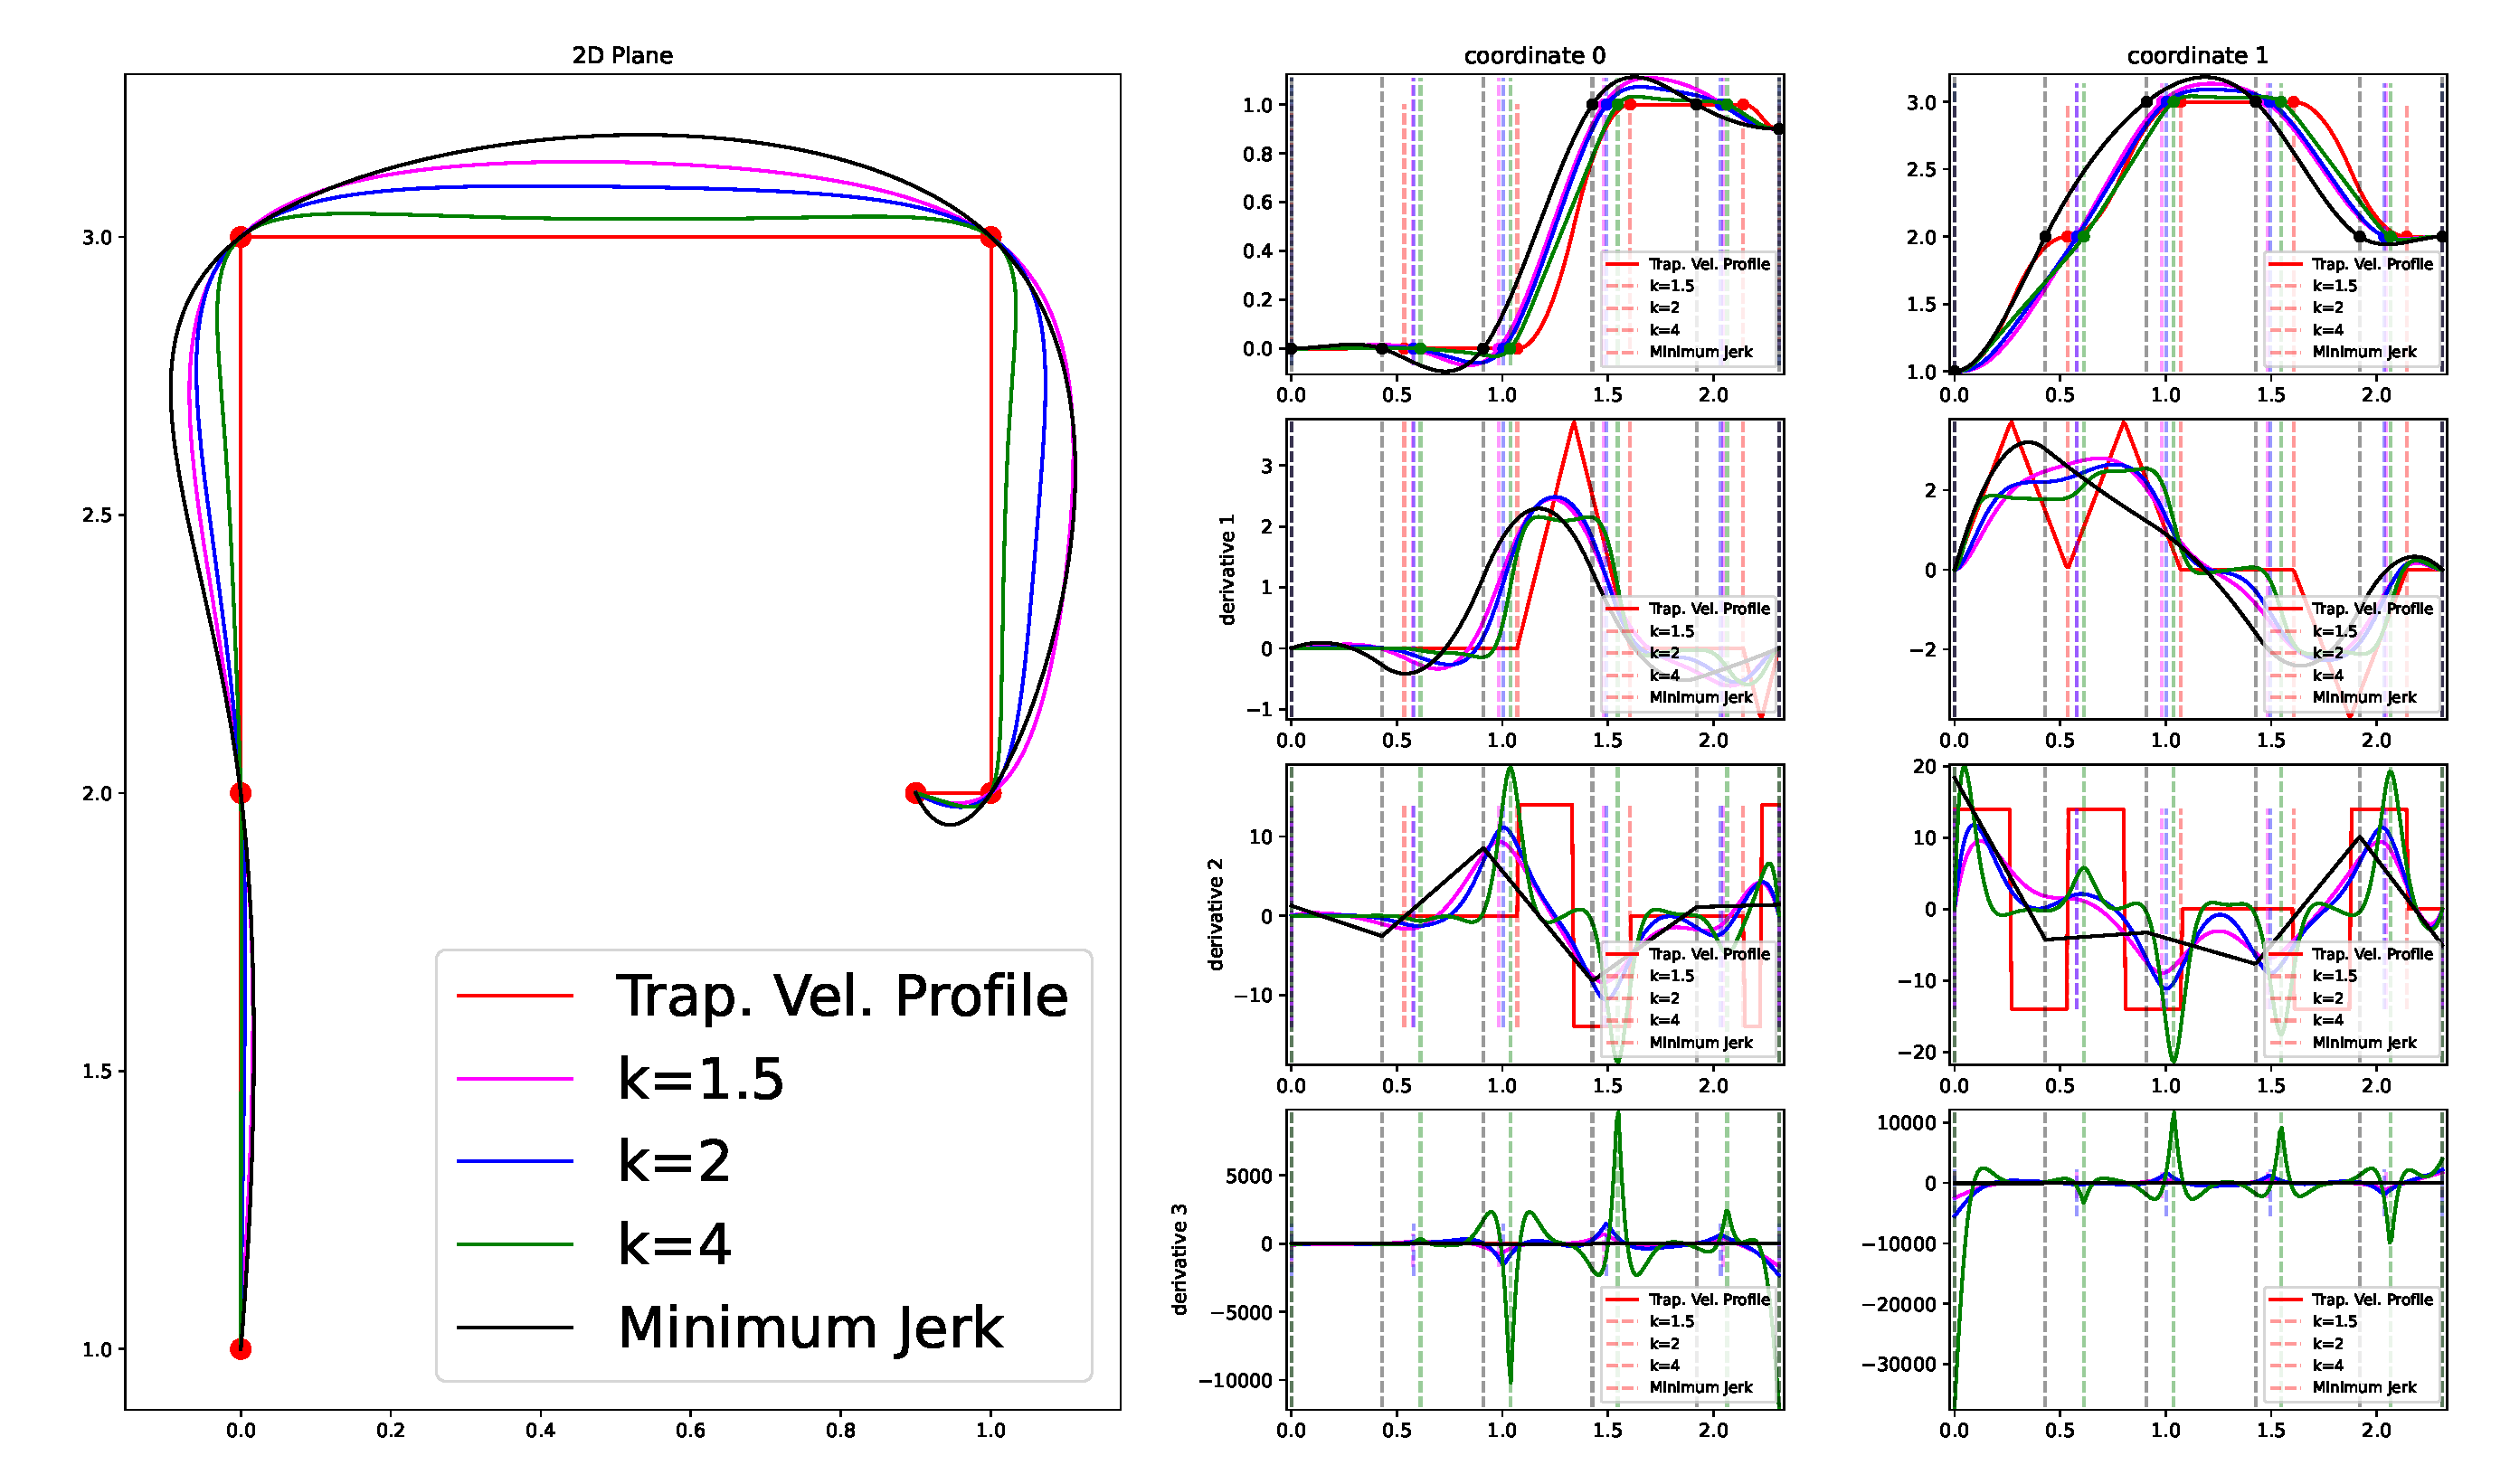
\includegraphics[width=10cm]{./images/kdl_comparision_2.pdf}};

		\node[anchor=west] (title) at (pic.east){%
			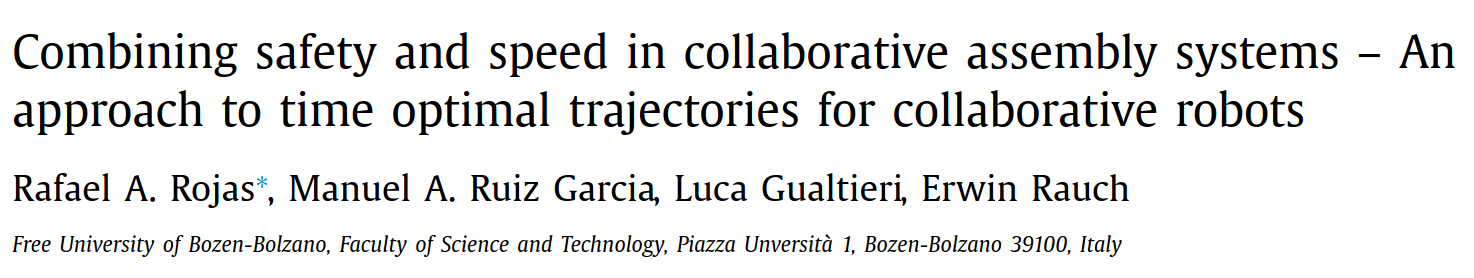
\includegraphics[width=5.5cm]{./images/reg_jerk_paper.png}};
		\node[anchor=south] (eq) at (title.north){%
			\parbox{5.5cm}{%
				\fontsize{9}{2}
				\begin{eqnarray*}
					\min \int_{t_0}^{t_f} \alpha \left\|\diffk{\qv}{t}{}\right\|^2  + (\alpha - 1 )\left\|\diffk{\qv}{t}{3}\right\|^2 \d t
				\end{eqnarray*}
			}
		};
		\node[anchor=north] at (title.south) {
			\parbox{5.5cm}{%
				\fontsize{9}{2}
				{\small Path shape parameter:}
				\begin{eqnarray*}
					k =  T\frac{\sqrt{2}}{4N}\sqrt[4]{\frac{\alpha}{1-\alpha}}.
				\end{eqnarray*}
			}
		};
	\end{tikzpicture}
\end{frame}
\begin{frame}
	\frametitle{Comparison with KDL Symmetric Velocity profiles}
	\framesubtitle{Speed comparison}
	\hglue -1cm
	\begin{tikzpicture}[scale=1]
		\node[anchor=north west](pic){%
			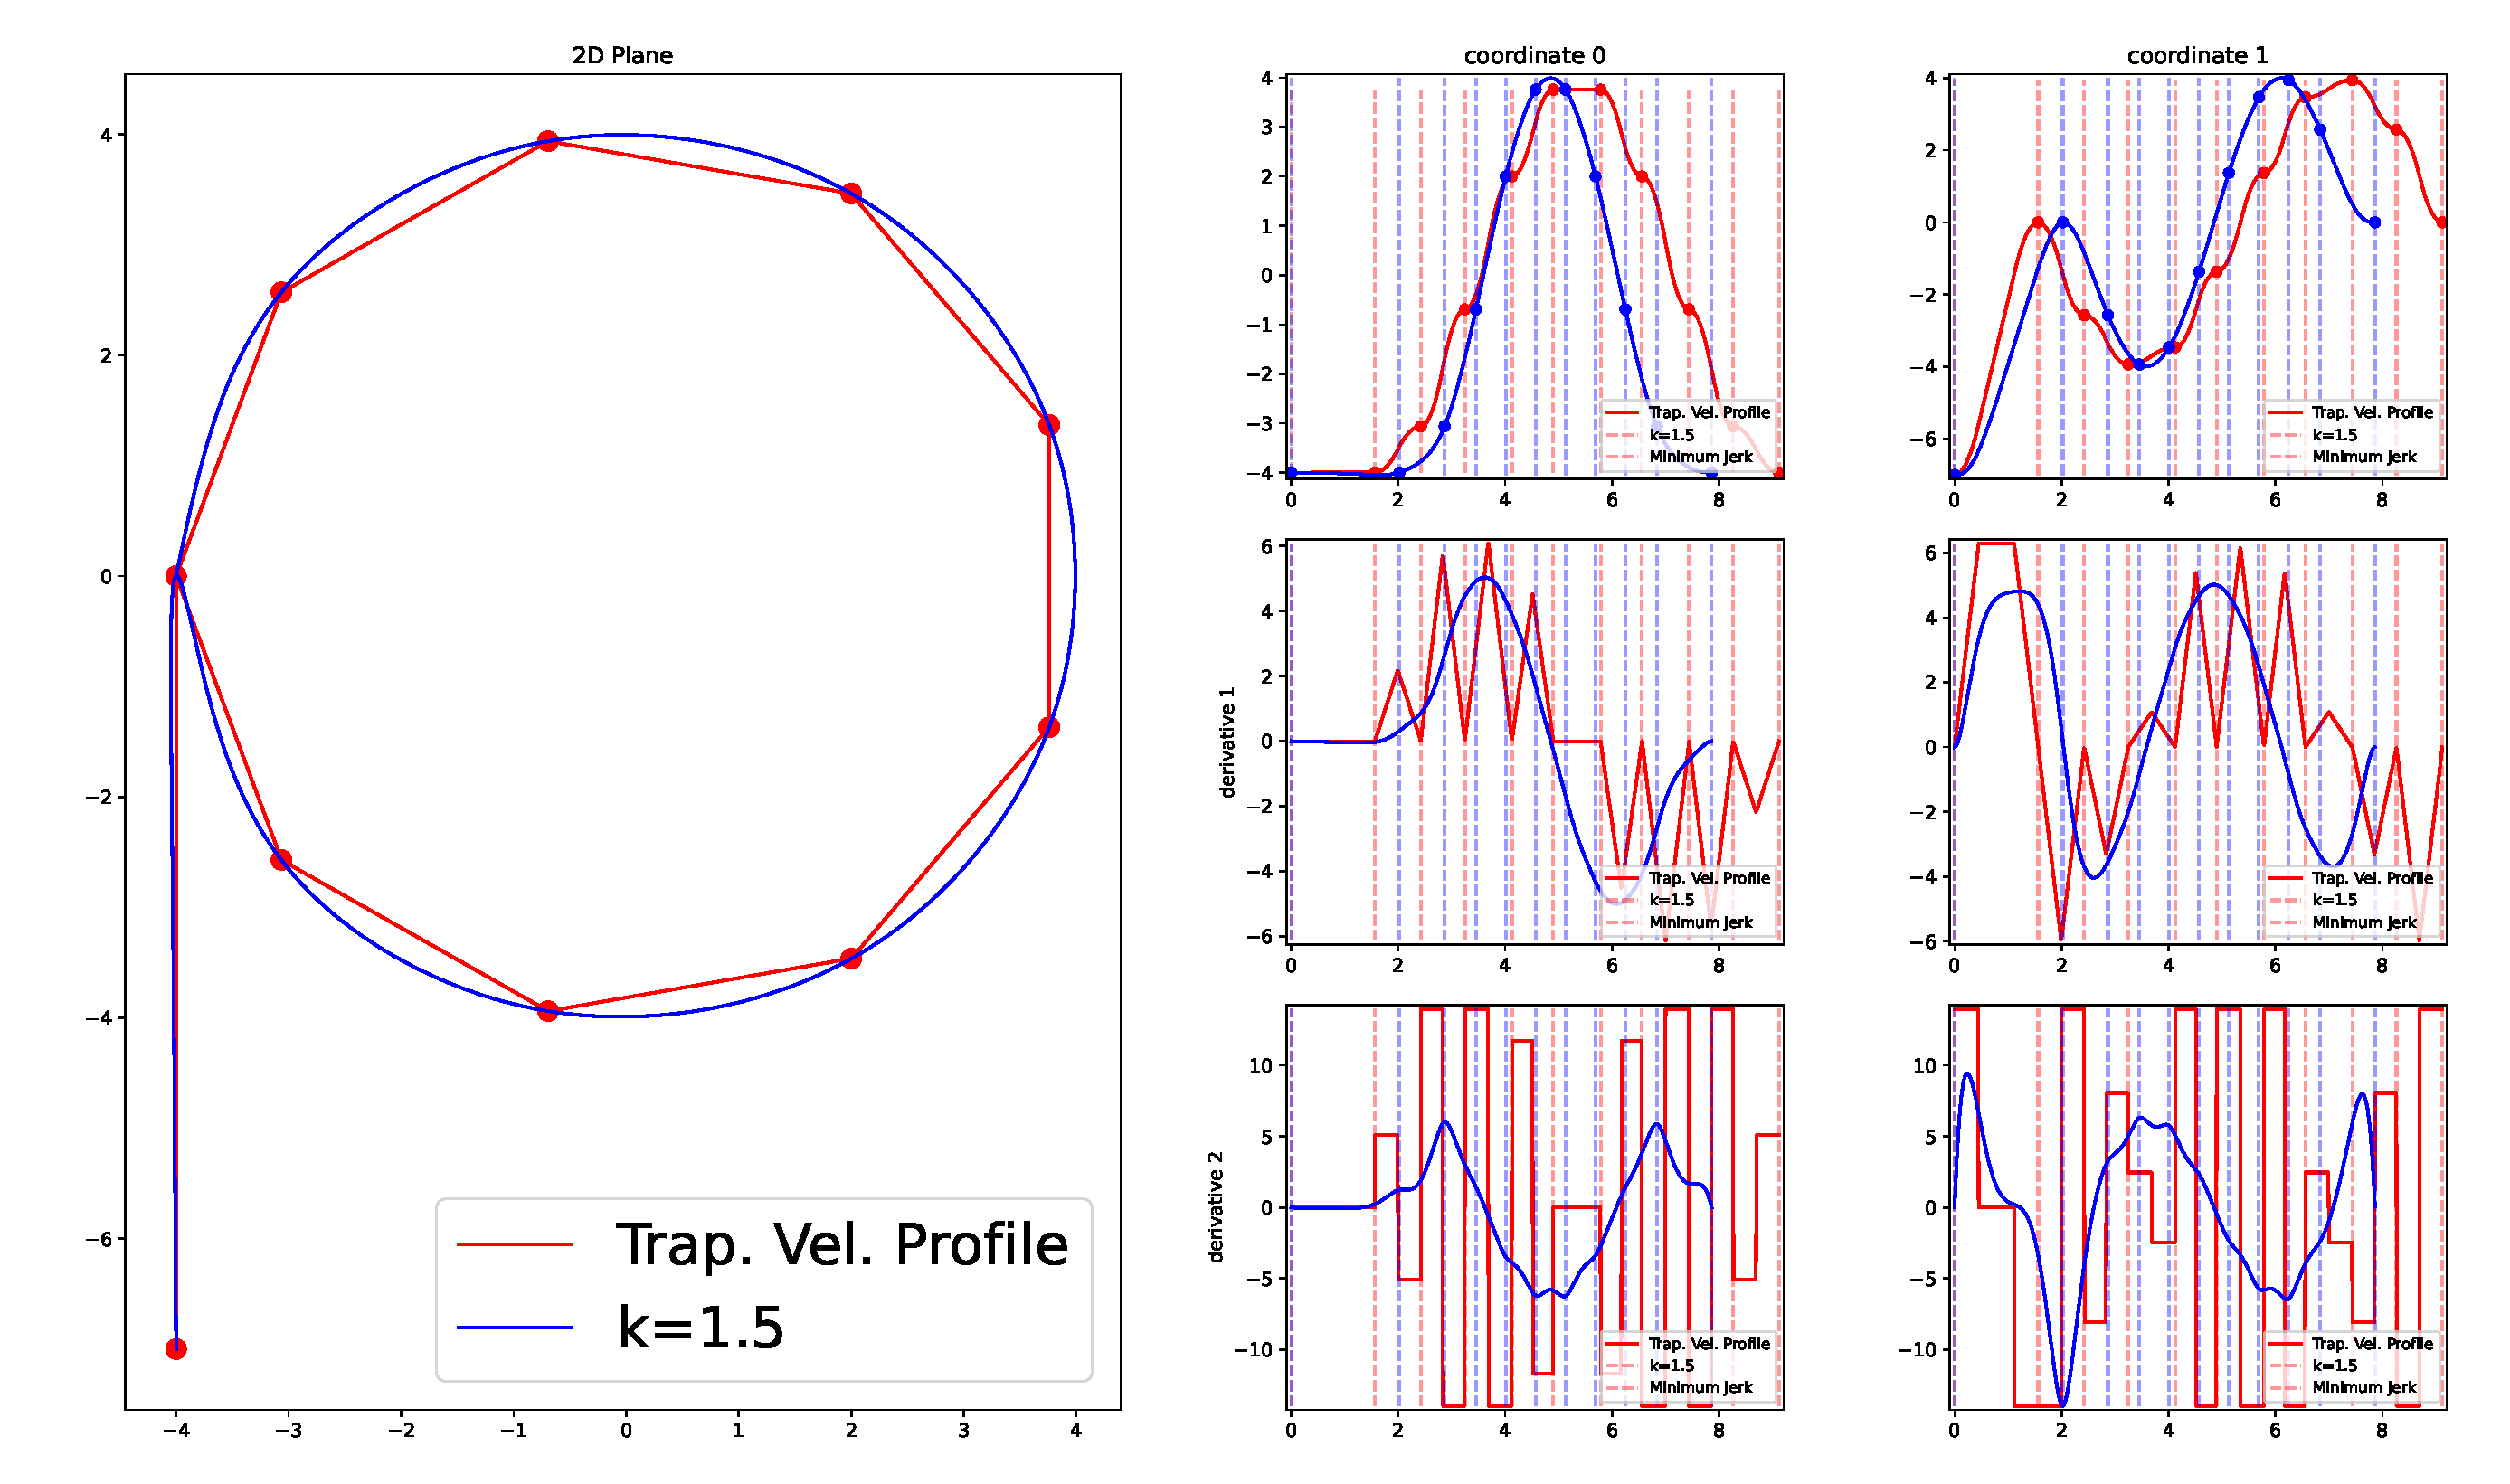
\includegraphics[width=10cm]{./images/kdl_speed_comparison.pdf}};
		\node[anchor=north west] (eq) at (pic.north east){%
			\parbox{5.5cm}{%
				\fontsize{9}{2}
				\begin{eqnarray*}
					\min \int_{t_0}^{t_f} \alpha \left\|\diffk{\qv}{t}{}\right\|^2  + (\alpha - 1 )\left\|\diffk{\qv}{t}{3}\right\|^2 \d t
				\end{eqnarray*}
			}};

		\node[anchor=west, node font=\fontsize{10}{10}\selectfont] (title) at (pic.east){\parbox{4cm}{
				\begin{itemize}
					\setlength{\itemsep}{1cm}
					\item 14\% Faster
					\item No blend radius
				\end{itemize}
			}};
	\end{tikzpicture}
\end{frame}

% \begin{frame}[fragile]
% 	\frametitle{Optimization: Interface}
% 	\begin{columns}
% 		\begin{column}{0.4\textwidth}
% 			\begin{itemize}
% 				\item By balancing the jerk with the velocity we can reduce these overshoots
% 				      \begin{equation*}
% 					      \min \int_0^T \alpha \diff{\qv}{t}  + (1-\alpha) \diffk{\qv}{t}{3} \d t
% 				      \end{equation*}
% 			\end{itemize}
% 			\begin{lstlisting}[language=python]

% waypoints = np.random.rand(4, 2)

% c1 = gsplines.optimization.broken_lines_path(waypoints)
% c3 = gsplines.optimization.minimum_jerk_path(waypoints)
% c4 = gsplines.optimization.rojas_path(waypoints, 0.8)
% c5 = gsplines.optimization.rojas_path(waypoints, 1.5)
% c6 = gsplines.optimization.rojas_path(waypoints, 2)

% gsplines.plot.plot2d_compare([c1, c3, c4, c5, c6], [
%             'green', 'blue', 'magenta', 'red',
%             'gray'],
%             ['min vel', 'min jerk', 'balance k=0.8',
%             'balance k=1.5', 'balance k=2'])
% \end{lstlisting}
% 		\end{column}
% 		\begin{column}{0.6\textwidth}
% 			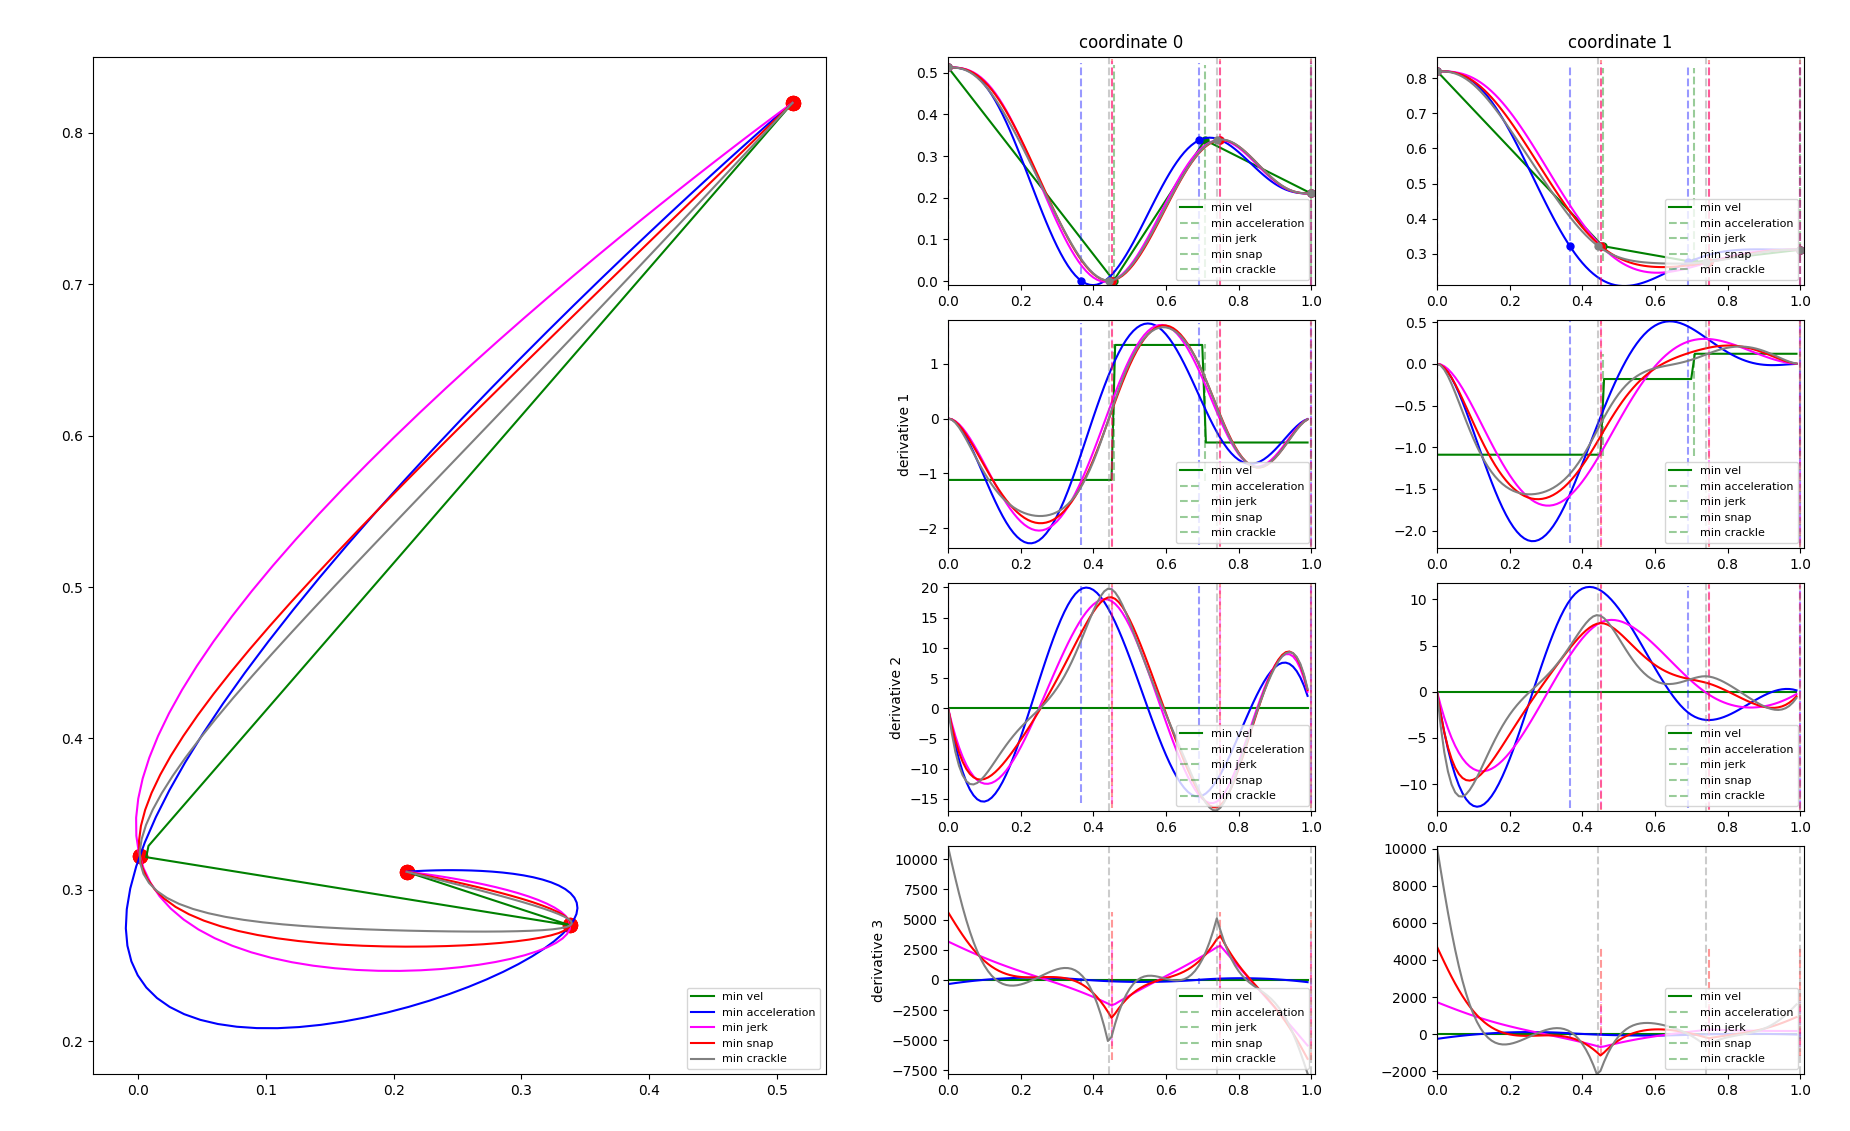
\includegraphics[width=\textwidth]{./images/comparison_2.png}
% 		\end{column}
% 	\end{columns}

% \end{frame}

